% This file was created by matplotlib2tikz v0.6.15.
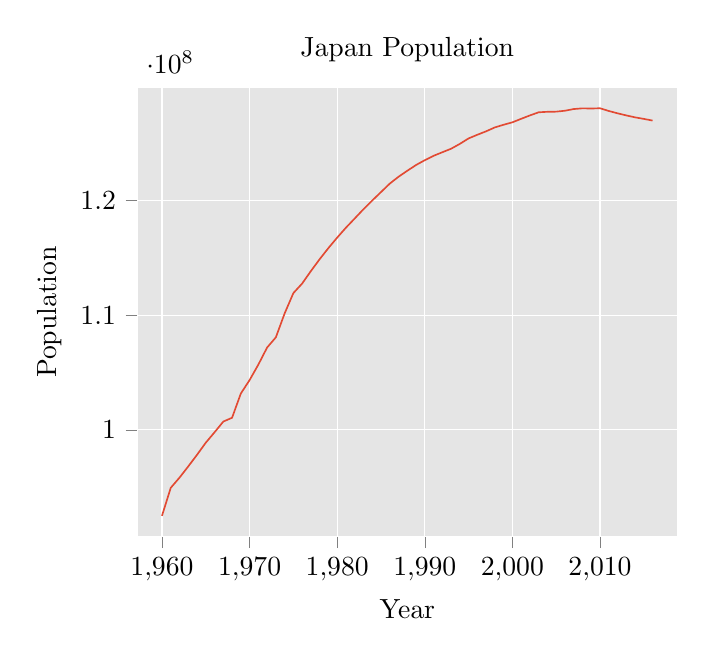
\begin{tikzpicture}

\definecolor{color0}{rgb}{0.886274509803922,0.290196078431373,0.2}

\begin{axis}[
title={Japan Population},
xlabel={Year},
ylabel={Population},
xmin=1957.2, xmax=2018.8,
ymin=90722100.6, ymax=129848471.4,
tick align=outside,
tick pos=left,
xmajorgrids,
x grid style={white},
ymajorgrids,
y grid style={white},
axis line style={white},
axis background/.style={fill=white!89.80392156862746!black}
]
\addplot [semithick, color0, forget plot]
table {%
1960 92500572
1961 94943000
1962 95832000
1963 96812000
1964 97826000
1965 98883000
1966 99790000
1967 100725000
1968 101061000
1969 103172000
1970 104345000
1971 105697000
1972 107188000
1973 108079000
1974 110162000
1975 111940000
1976 112771000
1977 113863000
1978 114898000
1979 115870000
1980 116782000
1981 117648000
1982 118449000
1983 119259000
1984 120018000
1985 120754000
1986 121492000
1987 122091000
1988 122613000
1989 123116000
1990 123537000
1991 123921000
1992 124229000
1993 124536000
1994 124961000
1995 125439000
1996 125757000
1997 126057000
1998 126400000
1999 126631000
2000 126843000
2001 127149000
2002 127445000
2003 127718000
2004 127761000
2005 127773000
2006 127854000
2007 128001000
2008 128063000
2009 128047000
2010 128070000
2011 127833000
2012 127629000
2013 127445000
2014 127276000
2015 127141000
2016 126994511
};
\end{axis}

\end{tikzpicture}